\documentclass[10pt,twocolumn,letterpaper]{article}

\usepackage{iccv}
\usepackage{times}
\usepackage{epsfig}
\usepackage{graphicx}
\usepackage{amsmath}
\usepackage{amssymb}
\usepackage{float}
\usepackage{subfigure}
\usepackage{array}
\usepackage{multirow}
% \usepackage{subcaption}

% Include other packages here, before hyperref.

% If you comment hyperref and then uncomment it, you should delete
% egpaper.aux before re-running latex.  (Or just hit 'q' on the first latex
% run, let it finish, and you should be clear).
\usepackage[pagebackref=true,breaklinks=true,letterpaper=true,colorlinks,bookmarks=false]{hyperref}

\newcommand{\PreserveBackslash}[1]{\let\temp=\\#1\let\\=\temp}
\newcolumntype{C}[1]{>{\PreserveBackslash\centering}p{#1}}
% \renewcommand\thesubfigure{(\alph{subfigure})}

\def\comm[#1]{{\small \textcolor{red}{\emph{#1}}}}
\def\red[#1]{\textcolor{red}{\textbf{#1}}}
\def\redn[#1]{\textcolor{red}{#1}}
\def\blue[#1]{\textcolor{blue}{#1}}
\def\green[#1]{\textcolor{green}{#1}}
\def\revise[#1]{{\small \textcolor{blue}{\emph{}}}}

% \iccvfinalcopy % *** Uncomment this line for the final submission

\def\iccvPaperID{612} % *** Enter the ICCV Paper ID here
\def\httilde{\mbox{\tt\raisebox{-.5ex}{\symbol{126}}}}

% Pages are numbered in submission mode, and unnumbered in camera-ready
\ificcvfinal\pagestyle{empty}\fi
\begin{document}

%%%%%%%%% TITLE
\title{Face Sketch Synthesis by Style Transfer with Local Features}

\author{First Author\\
Institution1\\
Institution1 address\\
{\tt\small firstauthor@i1.org}
% For a paper whose authors are all at the same institution,
% omit the following lines up until the closing ``}''.
% Additional authors and addresses can be added with ``\and'',
% just like the second author.
% To save space, use either the email address or home page, not both
\and
Second Author\\
Institution2\\
First line of institution2 address\\
{\tt\small secondauthor@i2.org}
}

\maketitle
%\thispagestyle{empty}


%%%%%%%%% ABSTRACT
\begin{abstract}

Face sketch synthesis is challenging as it is difficult to generate sharp and detailed textures. In this paper, we propose a new framework based on deep neural networks. Imitating the process of how artists draw sketches, our framework synthesizes face sketches in a cascaded manner in which a content image is first generated that outlines the shape of the face and key facial features, and textures and shadings are then added. We utilize a Fully Convolutional Neural Network (FCNN) to create the content image, and propose a local feature based style transfer to append textures. The local feature, what we call pyramid column feature, is a set of features at different convolutional layers corresponding to the same local sketch image patch. We demonstrate that our pyramid column feature can not only preserve more sketch details than common style transfer method but also surpass traditional patch based approach. Our model is trained and evaluated on CUHK and AR datasets. Quantitative and qualitative evaluations suggest that our framework outperforms other state-of-the-arts methods. In addition, despite of the small training data, our model shows great generalization ability across different datasets and can generate reasonable results under practical situations.

\end{abstract}

%%%%%%%%% BODY TEXT
%==========================================================================
\section{Introduction}

Face sketch synthesis has drawn a great attention from the community in recent years because of its wide range of applications. For instance, it can be exploited in law enforcement for identifying suspects from a mug shot database consisting of both photos and sketches. Besides, face sketch has also been widely used for entertainment purpose. For example, filmmakers could employ face sketch synthesis technique to ease the cartoon production process.

\begin{figure}[t]
\centering
\subfigure[Photo]{
\label{fig:example_a}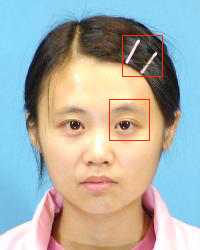
\includegraphics[width=0.23\linewidth]{img/page1_example/example_photo.png}}
\subfigure[MRF \cite{wang2009face}]{
\label{fig:example_b}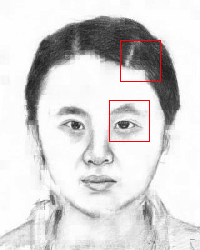
\includegraphics[width=0.23\linewidth]{img/page1_example/example_mrf.png}}
\subfigure[WMRF \cite{zhou2012markov}]{
\label{fig:example_c}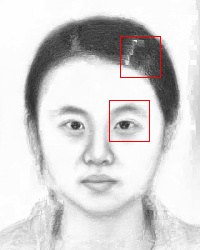
\includegraphics[width=0.23\linewidth]{img/page1_example/example_wmrf.png}}
\subfigure[SSD \cite{song2014real}]{
\label{fig:example_d}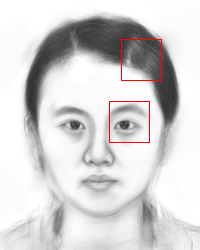
\includegraphics[width=0.23\linewidth]{img/page1_example/example_ssd.png}}
\subfigure[FCNN \cite{zhang2015end}]{
\label{fig:example_e}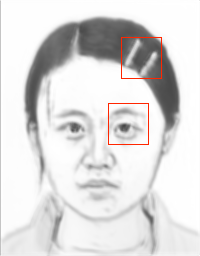
\includegraphics[width=0.23\linewidth]{img/page1_example/example_fcnn.png}}
\subfigure[BFCN \cite{zhang2017content}]{
\label{fig:example_f}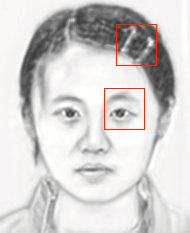
\includegraphics[width=0.23\linewidth]{img/page1_example/example_bfcn.png}}
\subfigure[\cite{gatys2015neural}$^*$]{
\label{fig:example_g}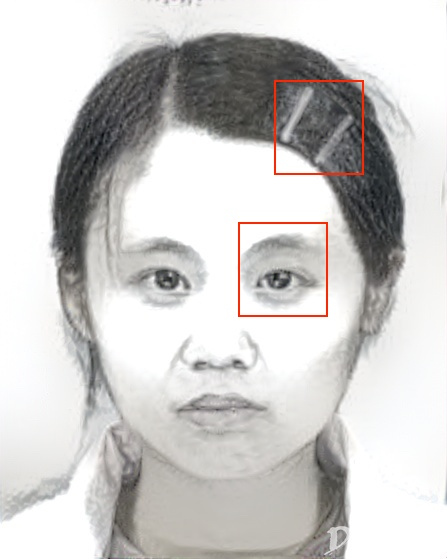
\includegraphics[width=0.23\linewidth]{img/page1_example/example_deepart.jpg}}
\subfigure[Ours]{
\label{fig:example_h}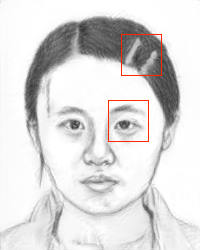
\includegraphics[width=0.23\linewidth]{img/page1_example/example_ours.png}}

\begin{minipage}[t]{1\linewidth}
\centering
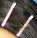
\includegraphics[width=0.11\linewidth]{img/page1_example/hairpin_photo_patch.png}
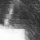
\includegraphics[width=0.11\linewidth]{img/page1_example/hairpin_mrf_patch.png}
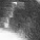
\includegraphics[width=0.11\linewidth]{img/page1_example/hairpin_wmrf_patch.png}
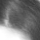
\includegraphics[width=0.11\linewidth]{img/page1_example/hairpin_ssd_patch.png}
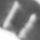
\includegraphics[width=0.11\linewidth]{img/page1_example/hairpin_fcnn_patch.png}
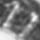
\includegraphics[width=0.11\linewidth]{img/page1_example/hairpin_bfcn_patch.png}
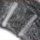
\includegraphics[width=0.11\linewidth]{img/page1_example/hairpin_deepart_patch.jpg}
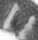
\includegraphics[width=0.11\linewidth]{img/page1_example/hairpin_ours_patch.png}
\end{minipage}
\begin{minipage}[t]{1\linewidth}
\centering
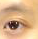
\includegraphics[width=0.11\linewidth]{img/page1_example/eye_photo.png}
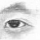
\includegraphics[width=0.11\linewidth]{img/page1_example/eye_mrf.png}
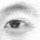
\includegraphics[width=0.11\linewidth]{img/page1_example/eye_wmrf.png}
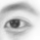
\includegraphics[width=0.11\linewidth]{img/page1_example/eye_ssd.png}
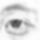
\includegraphics[width=0.11\linewidth]{img/page1_example/eye_fcnn.png}
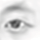
\includegraphics[width=0.11\linewidth]{img/page1_example/eye_bfcn.png}
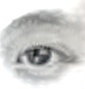
\includegraphics[width=0.11\linewidth]{img/page1_example/eye_deepart.jpg}
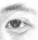
\includegraphics[width=0.11\linewidth]{img/page1_example/eye_ours.png}
\end{minipage}
\caption[Caption for LOF]{Face sketches generated by existing methods and the proposed method. Our method can not only preserve both hair and facial content, but also maintain sharp textures. \setcounter{footnote}{0} (h)$^*$ is obtained from deep art website\footnotemark~by using the photo as content and a sketch from training set as style.}
\label{fig:example_comp}
\end{figure}
\footnotetext{\url{https://deepart.io/}} 

Unfortunately, there exists no easy solution to face sketch synthesis due to the big stylistic gap between photos and sketches. In the past two decades, a number of exemplar based methods~\cite{wang2009face,song2014real, zhang2010lighting,zhou2012markov} were proposed. In these methods, an input photo is divided into patches and candidate sketches for each photo patch are selected from a training set. The main drawback of such kind of methods is that if the test image can't find a similar patch in the training set, they may lose some contents in the final result. For example, the sketches in the first row of Fig.\ref{fig:example_comp} fail to keep the hairpins. Besides, some methods \cite{song2014real,zhou2012markov} clear away the textures when they try to eliminate the inconsistency between neighboring patches. Another potential risk is that the result may not look like the original photo, \eg left eye in Fig.~\ref{fig:example_b}. Recently, approaches \cite{zhang2017content,zhang2015end} based on convolutional neural network (CNN) were developed to solve these problems. Since these models directly generates sketches from photo, they can maintain the structures and contents of the photos. However, the loss function of them are usually mean square error (MSE) or variation of it, which is responsible for the blur effect, \eg Fig.~\ref{fig:example_e} and ~\ref{fig:example_f}. The reason is that MSE prefers values close to mean, and is not suitable for texture representations. The popular neural style transfer provides a better solution for texture synthesis. But there are two obstacles towards directly applying such kind of method. First, it is easily influenced by illumination of the photo, see the face of Fig. \ref{fig:example_h}. Second, it needs a style image to give the global statistics of textures. If the given style doesn't coincide with target sketch (which we don't have), some side effects will occur, \eg the nose in Fig. \ref{fig:example_h}. Extensive experiment and discussion is given in Section~\red[??]. 

For an artist, the procedure of sketching a face usually starts with outlining the shape of the key facial features like the nose, eyes and mouth. Textures and shadings are then added to regions such as hair lips, and bridge of the nose to give sketches a specific style. Inspired by this and neural style transfer \cite{gatys2015texture}, we propose a new framework for face sketch synthesis that can overcome the aforementioned limitations. In our method, the outline of a face is delineated by a feed-forward neural network, and textures and shadings are then added by a style transfer approach. Specifically, we design a new architecture of Fully Convolutional Neural Network (FCNN) which contains inception layers \cite{szegedy2015going} and convolution layers with batch normalization~\cite{Sergey2015batch} to outline the face (Section ~\red[??]). For the texture part, we first divide the feature maps of the target sketch in each layer into a fixed size grid and combine features from different layers but at the same grid location into a pyramid feature column (Section ~\red[??]). These pyramid feature columns can be generated by local sketch patches from the training set. A target style is then computed by assembling these pyramid columns. These sketch patches are found by matching the test image patch to the image-patch pairs in training set(Section ~\red[??]). Our approach is superior to the current state-of-the-art methods in that 
\begin{itemize}
\item It is capable of generating more stylistic sketches without introducing over smoothing artifacts 
\item It can well preserve the content of the test photo.
\end{itemize}

%==========================================================================
\section{Related Work}\label{sec:related_work}

\subsection{Face Sketch Synthesis}

Based on the taxonomy of previous studies~\cite{song2014real,zhou2012markov}, face sketch synthesis methods can be roughly categorized into profile sketch synthesis methods~\cite{berger2013style,chen2001example,xu2008hierarchical} and shading sketch synthesis methods~\cite{liu2005nonlinear,song2014real,tang2003face,wang2009face,zhang2015end,zhang2010lighting,zhou2012markov}. Compared with profile sketches, shading sketches are more expressive and thus more preferable in practice. Based on the assumption that there exists a linear transformation between a face photo and a face sketch, the method in~\cite{tang2003face} computes a global eigen-transformation for synthesizing face sketches from face photos. This assumption, however, does not always hold since the modality of face photos and that of face sketches are quite different. Fortunately, Liu et al.~\cite{liu2005nonlinear} found that the linear transformation holds better locally and therefore they proposed a patch based method to perform sketch synthesis. A MRF based method~\cite{wang2009face} was proposed to preserve large scale structures across sketch patches. Variants of the MRF based methods were introduced in~\cite{zhang2010lighting,zhou2012markov} to improve the robustness to lighting and pose, and to render the ability of generating new sketch patches. In addition to these MRF based methods, approaches based on guided image filtering~\cite{song2014real} and feed-forward convolutional neural network~\cite{zhang2015end} are also found to be effective in transferring photos into sketches. A very recent work similar to ours is done by Zhang \etal \cite{zhang2017content}. They proposed a two branch FCNN to learn content and texture respectively and then fusion them through a face probability map. Although their results are impressing, the sketch texture is not natural and the facial components are smoothed.

%------------------------------------------------------------------------
\subsection{Style Transfer with CNN}

Texture synthesis has long been a challenging task. Traditional method can only imitate repetitive patterns which has a strong limitation. Recently, Gatys \etal ~\cite{gatys2015texture,gatys2015neural}, studied the use of CNN in style representation (including texture and color) where a target style is computed based on features extracted from an image using the VGG-Network and an output image is generated by minimizing the difference between its style and the target style. It can transfer any style to any images, and the results are impressive. Justin \etal \cite{feifei2016} further accelerated this process by learning a feed forward CNN in the training stage. These methods represent textures by a multi-scale gram matrix of feature maps. Since gram matrix cares more about global statistics, if the style is very different from the photo, it usually breaks the local structures. Although it is not a big deal in artistic style, it can't be tolerated in face sketch synthesis. In \cite{Chen2016Patch}, Chen and Schmidt propose a different patch based style transfer method which is better at capture local structures. However, it is still not suitable for this task. Our style transfer mechanism is inspired by but different from these works~\cite{gatys2015texture,gatys2015neural,feifei2016} in that our target style is extracted from many image patches rather than from a single style image. Note that there usually does not exist a single style image in the training set that matches all properties of the test image. 

\begin{figure*}[t]
\centering
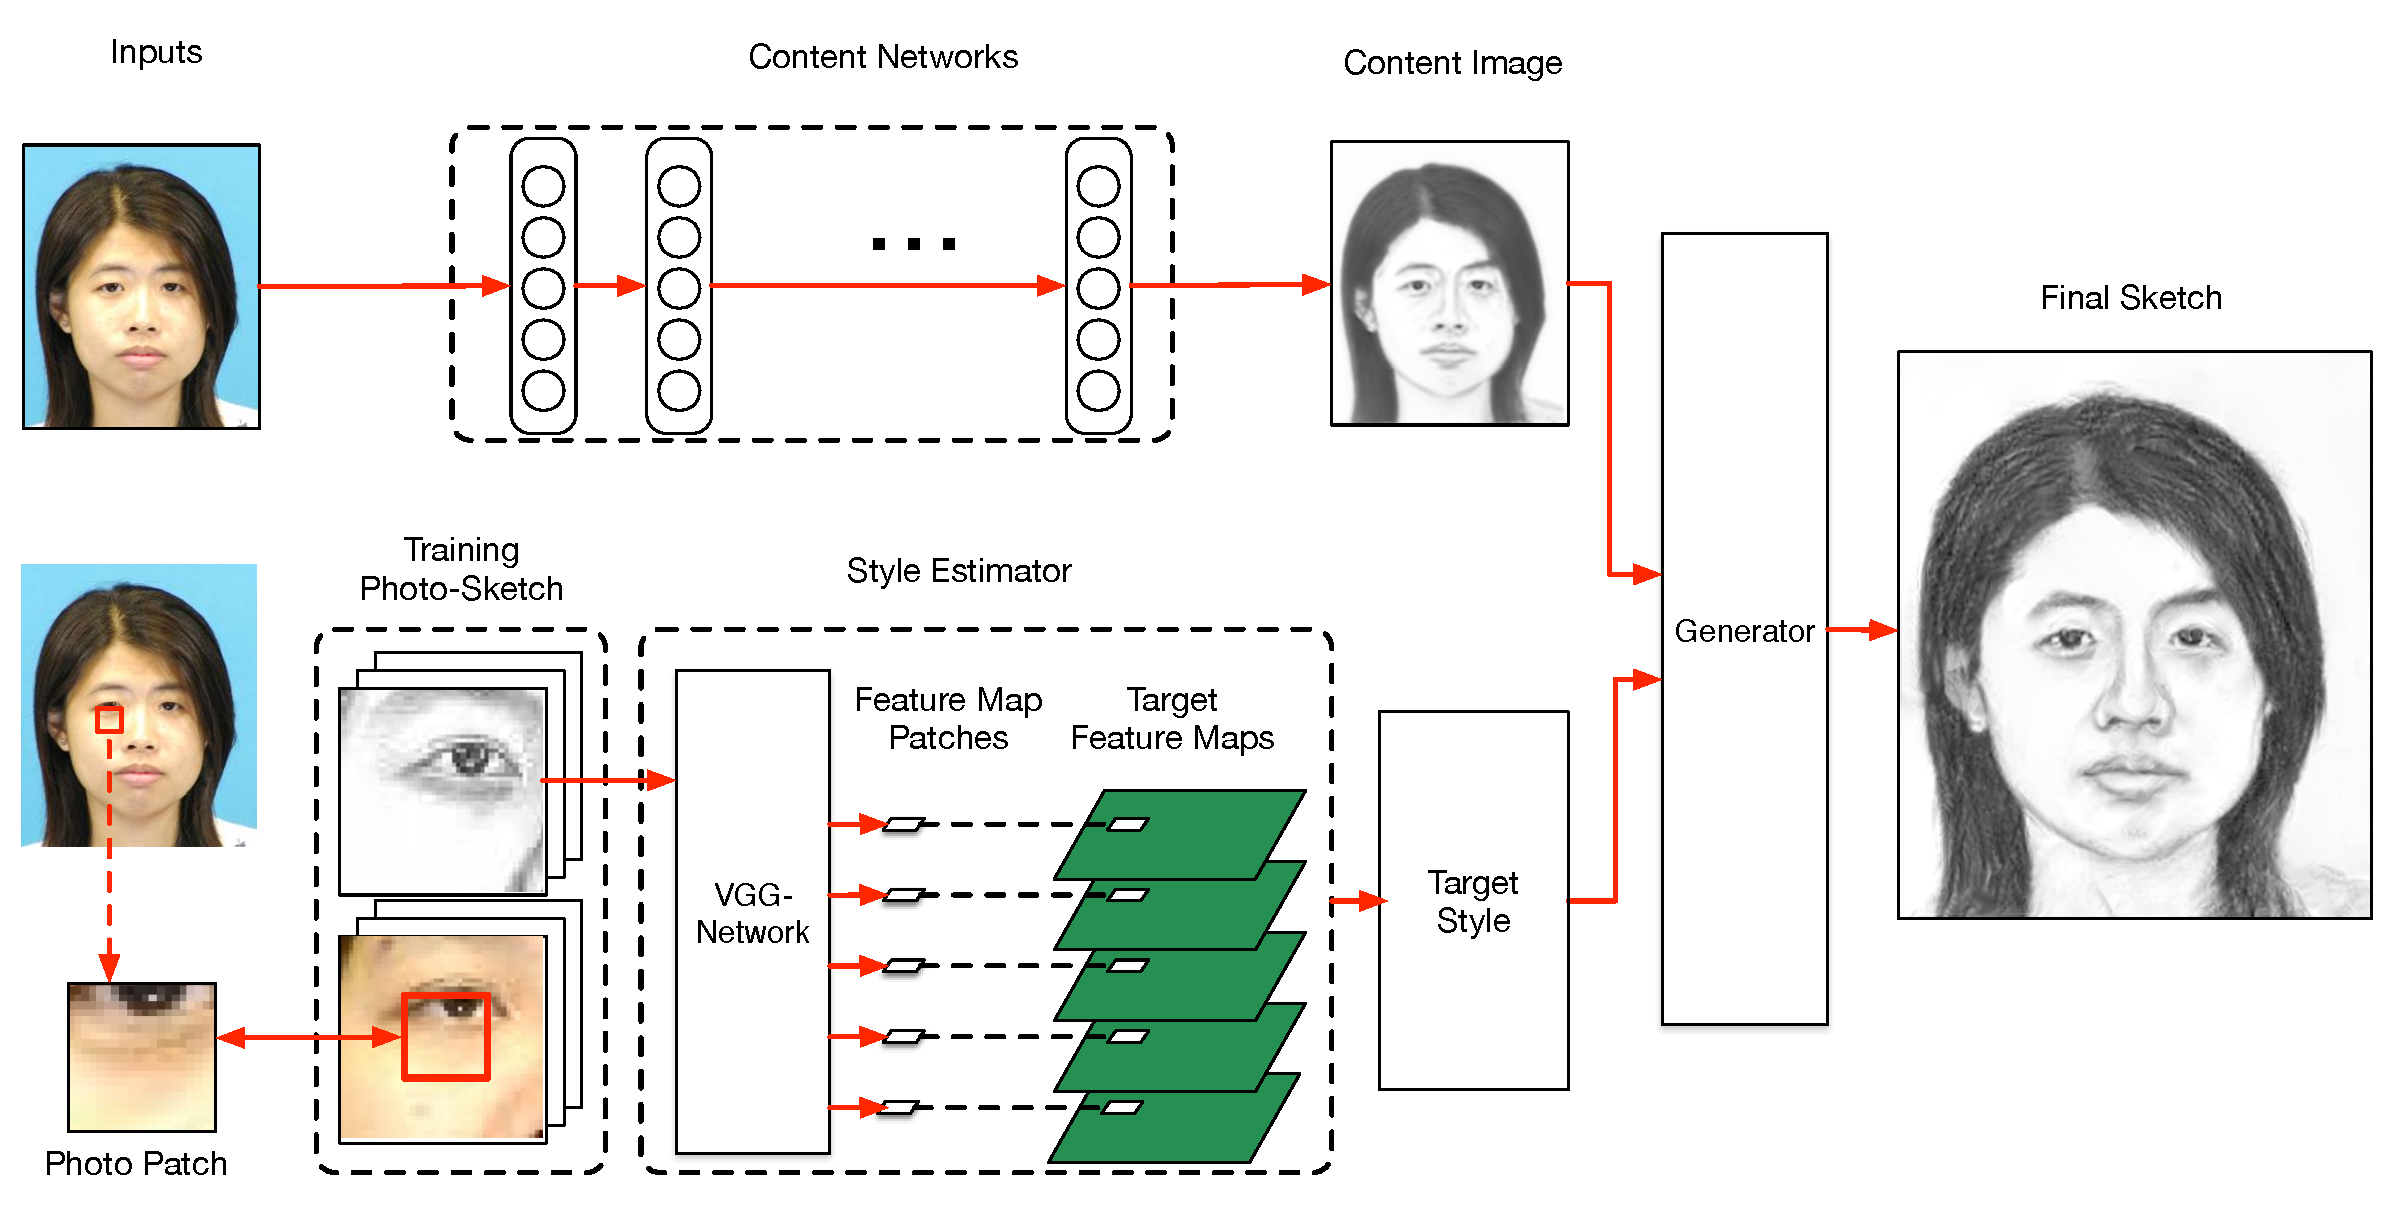
\includegraphics[width=0.85\linewidth]{img/overview.pdf}
\caption{The proposed method contains two branches which take an photo aligned by the eyes as inputs. The content network outputs a content image and the style estimator generates a target style. The final sketch is generated by combing the target style with the content image. \comm[The figure may need to revise, in order to show the optimization process of target sketch.]}
\label{fig:overview}
\end{figure*}
%==========================================================================
\section{Motivation of Pyramid Feature Column}\label{sec:motivation}

Following the practice of \cite{gatys2015neural}, we use the gram matrix of VGG-19\cite{simonyan2014very} feature maps as our style representation. Denote the vectorized feature map of the final sketch $\mathcal{X}$ in the $l$th layer by $F^{l}(\mathcal{X})$. A gram matrix is the inner product between the feature maps in $l$th layer
\begin{equation}
G^l_{ij}(\mathcal{X}) = \sum \limits_{k=1}^{M_l} F^l_{ik}(\mathcal{X}) F^l_{jk}(\mathcal{X})
\label{eq:Gram_element}
\end{equation}
where $G^l(\mathcal{X}) \in {\mathcal{R}^{N_l \times N_l}}$, $M_l$ is the height times width of the feature map $F^{l}(\mathcal{X})$, and $N_l$ is the number of feature maps in the $l$th layer. Since $G^l_{ij}(\mathcal{X})$ is an inner product of feature maps, a gram matrix is actually a summary statistics of feature maps discarding the spatial information. Although we still not clear what these values exactly mean, we can safely make an assumption that it at least captures the density distribution of a sketch. In other word, if the given sketch style has much less hair than the test image, the generated sketch $\mathcal{X}$ will possibly be unnaturally bright than a natural sketch. Experiments in Section~\red[??] also prove this. 
Thus it is important to keep the given style sketch roughly the same with test image statistically. On the other hand, there usually does not exist a candidate image in the training set that perfectly matches a given test photo in style. We hence propose a feature level patch based method to estimate the style of the final sketch. Each feature patch corresponds to a sketch patch. The reason why we can separate features into patches comes from \cite{Li2017Demistify}. The feature vectors at different position of feature map can be viewed as independent samples when we use gram matrix. 

%==========================================================================
\section{Methodology}

Our method can be classified as a shading synthesis method. The steps of our method are summarized in Fig.~\ref{fig:overview}. First, a preprocessing step as described in~\cite{wang2009face} is carried out for all photos and sketches in a training set to align the centers of two eyes. A test photo $\mathcal{I}$ is then fed into two branches, namely the content network and the style generator. The content network converts the test photo into a content image $\mathcal{C}$, where the shape of the face are outlined with the key facial features preserved, such as noses, eyes, mouthes and hair. The style estimator takes a $16\times16$ local patch from test photo as input and searches photo-sketch pairs in the training set to find a target sketch patch $S_{ij}$ ($(i, j)$ denotes the patch location). Each  $S_{ij}$ with its surrounding region can generate a pyramid feature column $U_{ij}$. Combining all $U_{ij}$, we can get the target style features of $\mathcal{I}$, \ie $\tilde{U}$. Given $\mathcal{C}$ and $\tilde{U}$, we can generate a sketch $\mathcal{X}$ that combines the content information in $\mathcal{C}$ with the style representation $\tilde{U}$ following the iterative procedure in \cite{gatys2015neural}. 

%------------------------------------------------------------------------
\subsection{Content Image Generation}
\begin{figure*}[htbp]
\centering
\subfigure[The architecture of content network]{
\label{fig:content_NN_a}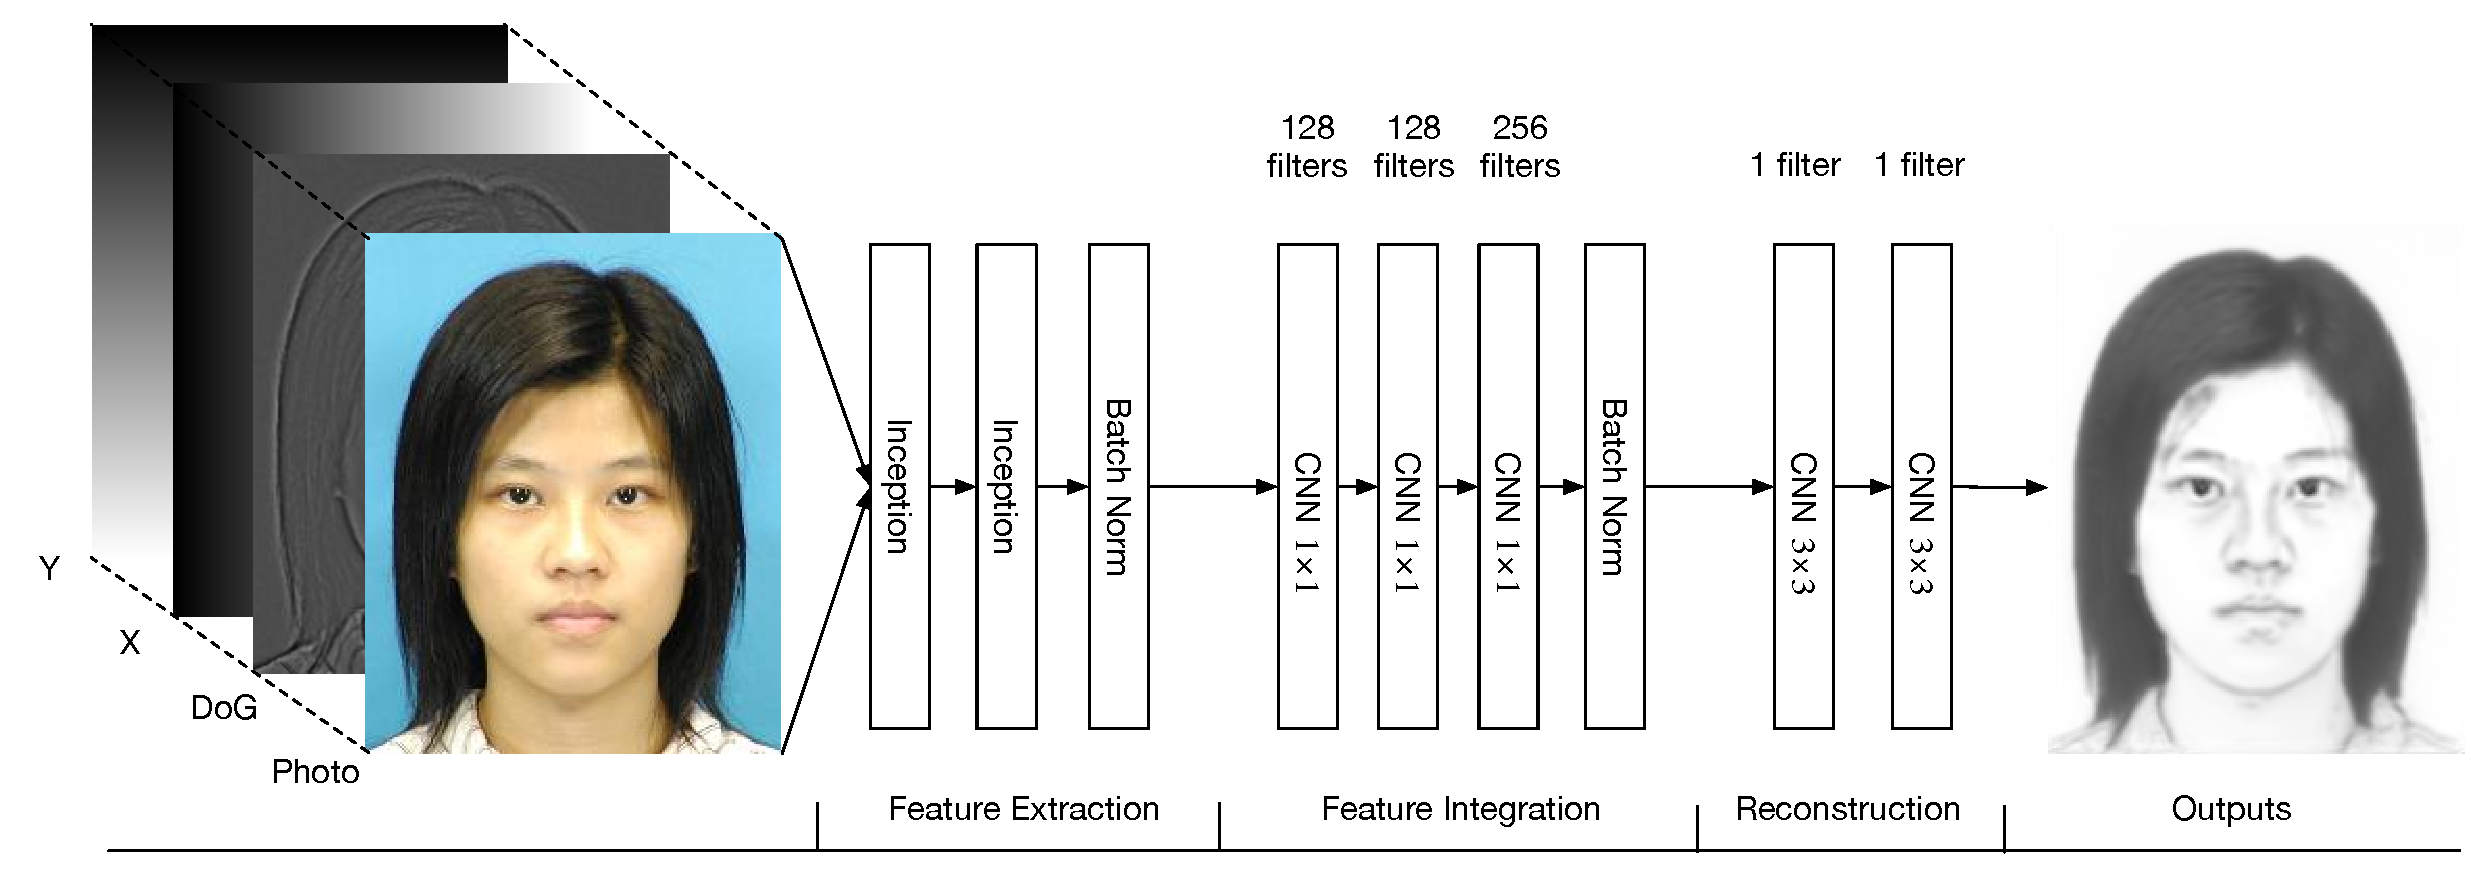
\includegraphics[width=0.65\linewidth]{img/content_net.pdf}}
\subfigure[Inception module]{
\label{fig:content_NN_b}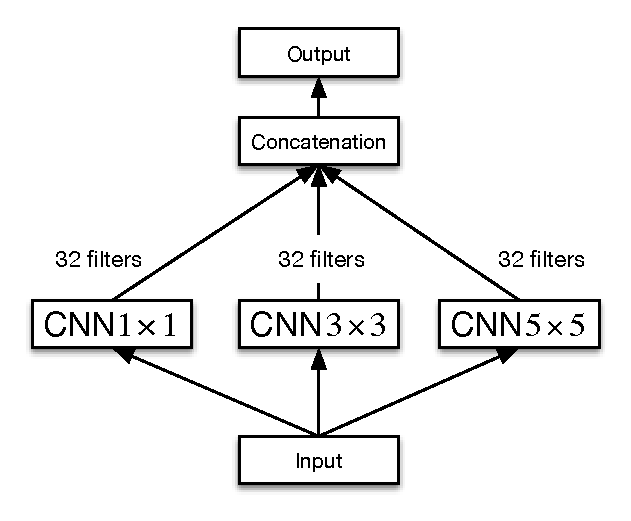
\includegraphics[width=0.25\linewidth]{img/inception.pdf}}
\caption{Illustration of the content network for generating a content image. The numbers above the building block denote the number of CNN filters. (a) The architecture of content network. (b) The inception module in (a) contains three groups of filters with different sizes.}
\label{fig:content_NN}
\end{figure*}

Our content network architecture is shown in Fig.~\ref{fig:content_NN}. In addition to the test photo, we feed two extra channels containing spatial information (i.e., x and y coordinates) and a difference of Gaussian (DoG) image into the content network. As pointed out in~\cite{wang2009face}, face sketch synthesis algorithms benefit from integrating features from multiple resolutions. We employ an inception module inspired by the GoogLeNet~\cite{szegedy2015going} to extract features. It concatenates feature maps generated from filters with different spatial resolutions. Our inception unit contains 3 different size of filters $(1\times1)$, $(3\times3)$ and $(5\times5)$ (see Fig. \ref{fig:content_NN_b}). Then, the output features are fed to a three-layer-CNN for feature integration, where the size of all filters are fixed at $1\times1$. Finally, the integrated features are used to reconstruct the content map by a two-layer-CNN with the filter size being $3\times3$. Because $L_1$-norm is better at preserving details than $L_2$-norm, we use the $L_1$-norm between the generated content image $\mathcal{C}$ and ground truth sketch $S$ as the loss function, see Equ.~\ref{eq:content-net-loss}.
\begin{equation}
\mathcal{L}_s = \frac{1}{N} \sum \limits_{i=1}^N \|\mathcal{C}_i - S_i\| \label{eq:content-net-loss}
\end{equation}
where $N$ is the number of photos. 

\subsection{Pyramid Feature Column}
%------------------------------------------------------------------------

Fig. \ref{fig:pyramidcolumn} shows an example of the pyramid feature column. Denote the feature maps (of the $l$th layer) used to estimate the style of the final sketch by $A^{l}$. In our feature patch based method, we divide $A^{l}$ into a fixed size of grid. Due to the different feature map size, the sizes of the feature patches at layer $conv1\_1$, $conv2\_1$, $conv3\_1$, $conv4\_1$ and $conv5\_1$ are $16\times16$, $8\times8$, $4\times4$, $2\times2$ and $1\times1$. The photos and sketches are resized to $288\times288$, thus the size of grid is $18\times18$. Grouping feature map patches having the same grid indexes $(i, j)$ at different layers together, we get a pyramid feature column $U_{ij}$. To estimate $U_{ij}$, a sketch patch in the training set is fed to the VGG-Network and a pyramid column is composed of the resulting feature maps. This process consists of two steps: (1) find a matching sketch patch $S_{ij}$ from the training set for $U_{ij}$ and (2) feed $S_{ij}$ to VGG-Network and extract $U_{ij}$ from the resulting feature maps.

\begin{figure}[htbp]
\centering
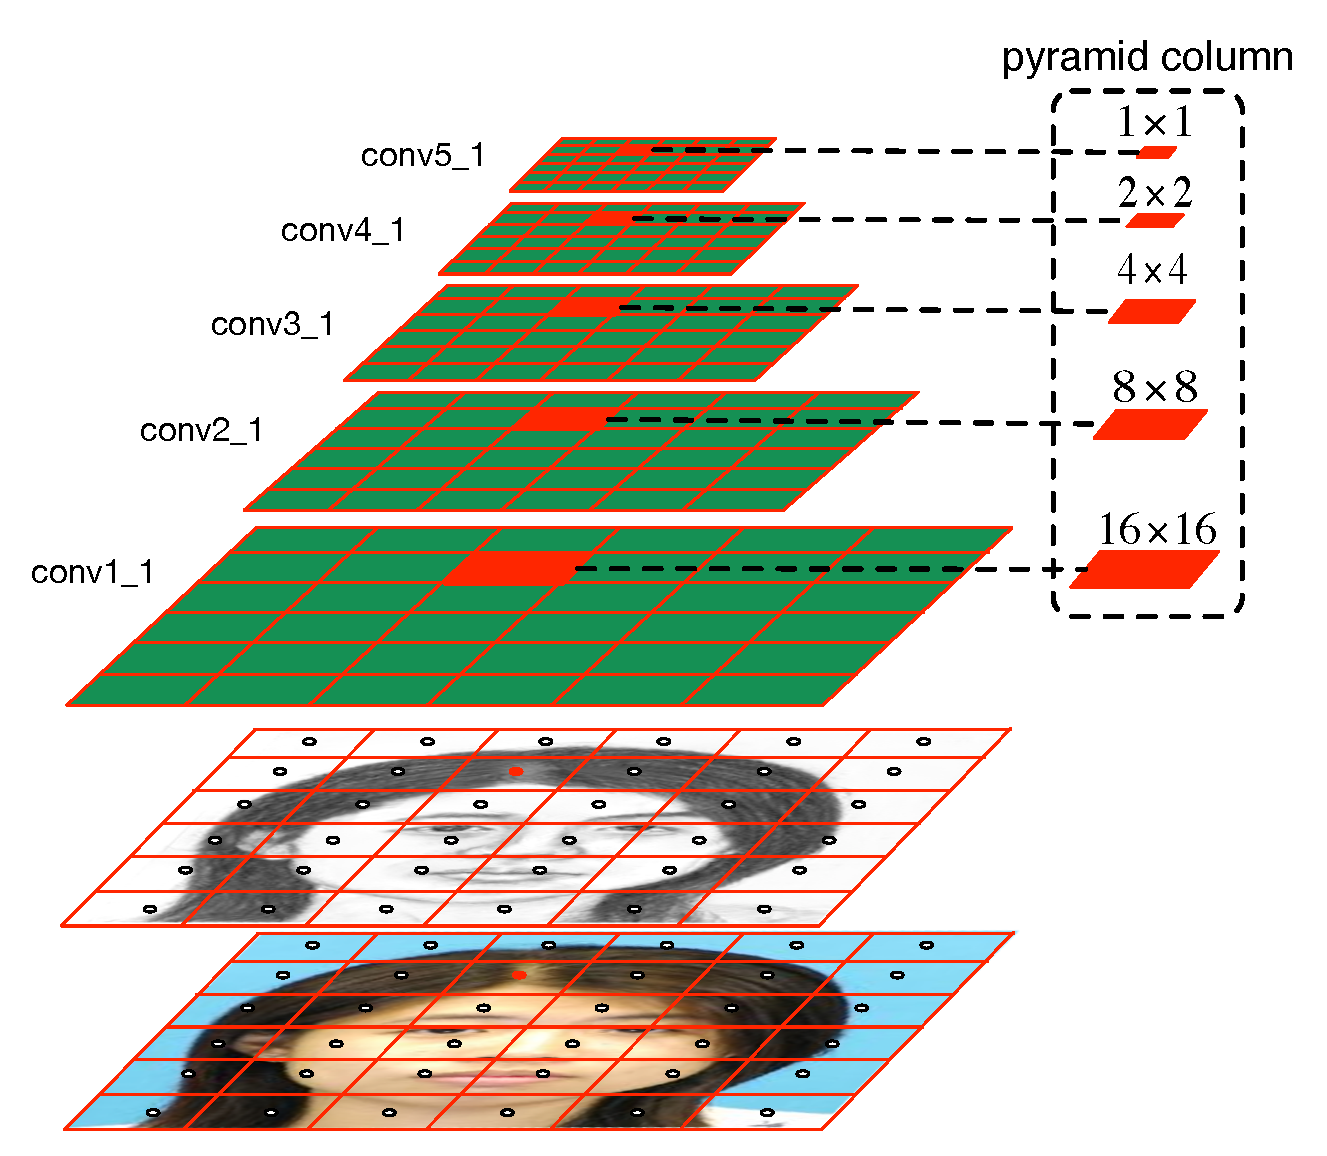
\includegraphics[width=0.85\linewidth]{img/pyramidcolumn.pdf}
\caption{Illustration of pyramid feature column. Feature maps of the final sketch $A^{l}$ are divided into a fixed $18\times18$ grid. A pyramid column $U_{ij}$ consists of feature map patches at different layer having the same grid indexes $(i, j)$.}
% The input photo and the final sketch are divided into patches where centers $C_{ij}$ are denoted as dots. $U_{12}$ and $C_{12}$ are colored in red as an example.
\label{fig:pyramidcolumn}
\end{figure}

\paragraph*{Find Matching Sketch Patch} Similar to previous works~\cite{wang2009face,zhou2012markov}, we examine the similarity of test photo patch and train photo patches to find a matching sketch $S_{ij}$ for $U_{ij}$. Denote the train photo patch set as $P$, given a test photo patch $T'_{ij}$, the target sketch patch $S'_{ij}$ is found by
\begin{gather}
S'_{ij} = \phi(\min_{T^k_{mn} \in P} f(T^k_{mn}, T'_{ij})) \\
m = i + \Delta x, n = j + \Delta y
\end{gather}
where $T^k_{mn}$ is the photo patch of the $k$th image at $(m, n)$ in training set, $\phi$ is a one-to-one mapping between photo patch and sketch patch, $\Delta x$ and $\Delta y$ is the shift of $(m, n)$ around $(i, j)$. The function $f$ measures the discrepancy between $T^k_{mn}$ and $T'_{ij}$. Because we only need the test photo patch and train photo patch have a similar appearance, we simply use MSE as $f$ here.

\paragraph*{Estimate Pyramid Feature Column}
After we get $S_{ij}$, we can compute the corresponding pyramid feature column $U_{ij}$. Although the feature column can be generated by a $16\times16$ patch, padding zeros is not a good idea. Therefore, we will make use of the surrounding area of $S_{ij}$ to compute $U_{ij}$. According to the architecture of VGG-19, the receptive field of $conv5\_1$ is 132 without padding. To get $16\times16$ patches, we will need a $144\times144$ region $\mathcal{R}$ containing 81 patches in total. $S_{ij}$ should be at the center of $\mathcal{R}$, \ie $S_{55}$ with respect to the grids of $\mathcal{R}$. For those border part where we can't find a region centered at $S_{ij}$, we just find another region $\mathcal{R}'$ which has the biggest intersection with the should be region $\mathcal{R}$ (the blue box in Fig. \ref{fig:border_example}). The $S_{55}$ in $\mathcal{R}$  should be $S'_{pq}$ in $\mathcal{R}'$ ($(p, q)$ is calculated according to different conditions). The feature column $U_{55}$ in $\mathcal{R}$ or $U_{pq}$ in $\mathcal{R'}$ is the estimated pyramid feature column. 

Allocating all these feature columns to its original patch location $(i, j)$, we can get the final feature maps $\tilde{U}$ and use it to compute gram matrix.  

\begin{figure}[htbp]
\centering
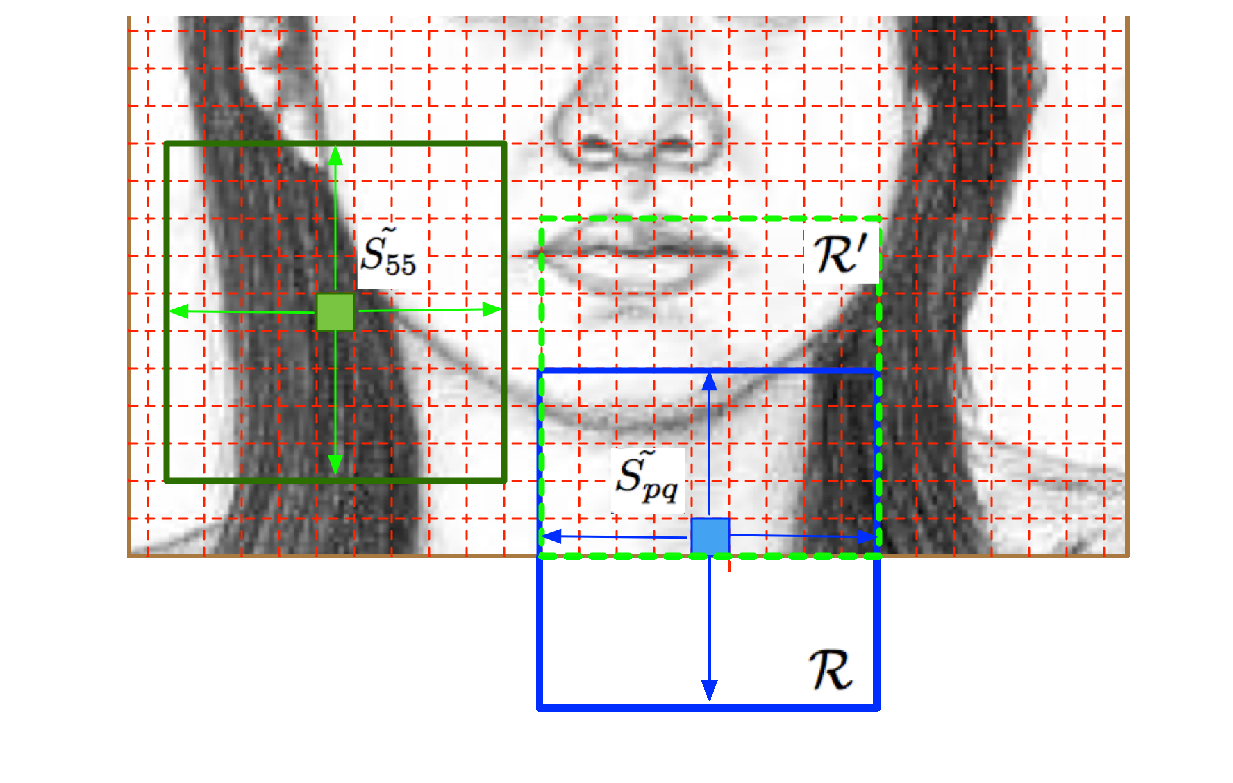
\includegraphics[width=0.99\linewidth]{img/border_PFC.eps}
\caption{Find a region $\mathcal{R}$ centered at $S_{ij}$. If $\mathcal{R}$ is inside the image, $S_{ij}$ should be the center patch of $\mathcal{R}$, see the left region. Otherwise, we need to find $\mathcal{R}'$ inside the image which has the biggest intersection with $\mathcal{R}$, see the right part. Suppose the indexes of $\tilde{S_{ij}}$ inside $\mathcal{R}'$ is $(p, q)$, then $U_{pq}$ is the corresponding feature column.}
\label{fig:border_example}
\end{figure}

\subsection{Loss Function of Sketch}

The same as \cite{gatys2015neural}, our loss function has a style loss and content loss. In addition we add a component loss to enhance the key facial components. The total loss is

\begin{equation}
\mathcal{L}_{t}( \mathcal{X} ) = \alpha \mathcal{L}_{c} + \beta_1 \mathcal{L}_{s} + \beta_2 \mathcal{L}_{k}
\label{eq:Total_loss}
\end{equation}
We minimize the loss function by updating the target sketch $\mathcal{X}$ without changing the VGG parameters.

The content loss is defined based on the difference between the feature map of the sketch and the content image at layer conv1\_1:
\begin{equation}
\mathcal{L}_{c}( \mathcal{X} ) = \| {{F^{\rm{conv1\_1}}}( \mathcal{X} ) - {F^{\rm{conv1\_1}}}( \mathcal{C} )} \|_2^2.
\label{eq:content_loss}
\end{equation}
And the style loss is the difference between the gram matrix of the final sketch and the target gram matrix 
\begin{equation}
\mathcal{L}_{s} ( \mathcal{X} ) = \sum\limits_{l \in {L_s}} {\frac{1}{{M_l^2N_l^2}}\| {{G^l}( \mathcal{X} ) - G^l(\tilde{U})} \|_2^2} 
\label{eq:Gram_loss}
\end{equation}
where $N_l$ denotes the number feature maps at layer $l$, and $M_l$ is the feature map width times height.  

To better transfer styles of the key facial components, we employ a component loss to encourage the key component style of the final sketch being the same as the target key component style. Since two eyes are placed at fixed positions, the key components lie roughly within a rectangular region taking the positions of two eyes as vertices. Key component style is given by gram matrices calculated within feature map regions $\mathcal K$ corresponding to the key components. These regions are specified by pyramid feature columns $U_{ij}$ whose $\mathcal{C}_{ij}$ are inside $\mathcal K$. We take out $\mathcal K$ and calculate the corresponding gram matrix loss as the component loss
\begin{equation}
\mathcal{L}_{k} ( \mathcal{X} ) = \sum\limits_{l \in {L_s}} {\frac{1}{{\hat{M}_l^2{N}_l^2}}\| {{{\hat G}^l}( \mathcal{K} ) - {\hat G}^l(\tilde{U}_k)} \|_2^2} 
\label{eq:component_loss}
\end{equation}
where $\hat{M}_l$ denotes height times width of $\mathcal K$. 

%------------------------------------------------------------------------
\subsection{Implementation Details}

\paragraph*{VGG-19 Parameters} Since the VGG-Network is originally designed for color images, while sketches are gray scale images, we modify the first layer of VGG-Network for gray scale images by setting the filter weights to
\begin{equation}
W^{k} = W^{k}_r+W^{k}_g+W^{k}_b
\label{eq:VGG_weights}
\end{equation}
where $W^{k}_r$, $W^{k}_g$, and $W^{k}_b$ are weights of the $k$th filter in the first convolutional layer for the R, G and B channels respectively, and $W^{k}$ is the weight of the $k$th filter in the first convolutional layer of our modified network.

\paragraph{Data Partition} CUHK has 88 training photos and 100 test photos, and AR has 123 photos. Our training set is composed of the 88 training photos of CUHK and 100 photos from AR. When training the content network, 10\% of the training set are taken out as validation set. All the 188 photo-sketch pairs are used to generate target sketch.

\paragraph{Training content network} The input photo-sketch pairs are aligned by the facial landmarks of eyes, and all images are resized to $200\times256$. A mirror padding is carried out before the convolution operation when necessary to ensure the output feature map is the same size as the input. Adadelta \cite{matt2012adadelta} is used as the optimizer because it is stable and much faster than others.  

\paragraph{Sketch Generation} 
In all experiments, we resize test photos and photo-sketch pairs in the training set to a fixed size of $288\times288$. The final sketch is obtained by resizing the resulting sketch back to the original size. The size of $\mathcal{K}$ is $48\times48$, $\alpha=0.004$, $\beta_1=1$ and $\beta_2=0.1$. The minimization is carried out using L-BFGS. Instead of using random noises, we use the content image as a starting point, which will make the optimization process converge much faster. 

%==========================================================================

\begin{figure*}[htbp]
\centering
\subfigure[Photo]{
\begin{minipage}[b]{0.1\linewidth}
\centering
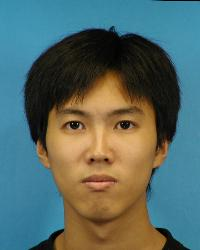
\includegraphics[width=0.91\linewidth]{img/sketch_result/example1_photo.png}
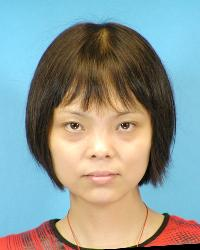
\includegraphics[width=0.91\linewidth]{img/sketch_result/example2_photo.png}
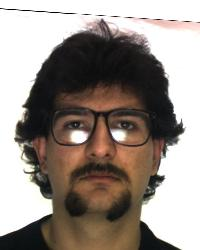
\includegraphics[width=0.91\linewidth]{img/sketch_result/example3_photo.png}
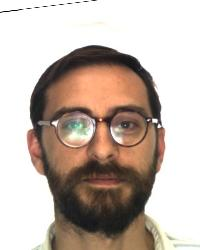
\includegraphics[width=0.91\linewidth]{img/sketch_result/example4_photo.png}
\end{minipage}
}
\subfigure[MRF]{
\begin{minipage}[b]{0.13\linewidth}
\centering
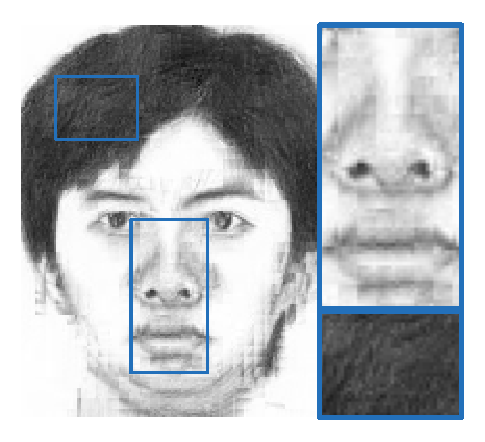
\includegraphics[width=0.99\linewidth]{img/sketch_result/example1_MRF.pdf}
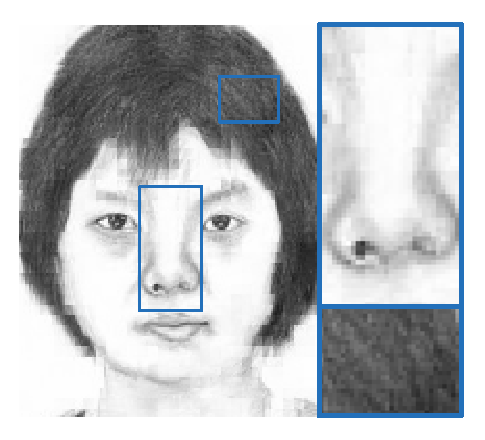
\includegraphics[width=0.99\linewidth]{img/sketch_result/example2_MRF.pdf}
% \includegraphics[width=0.99\linewidth]{img/sketch_result/example3_MRF.pdf}
% \includegraphics[width=0.99\linewidth]{img/sketch_result/example4_MRF.pdf}
\end{minipage}
}
\subfigure[WMRF]{
\begin{minipage}[b]{0.13\linewidth}
\centering
% \includegraphics[width=0.99\linewidth]{img/sketch_result/example1_WMRF.pdf}
% \includegraphics[width=0.99\linewidth]{img/sketch_result/example2_WMRF.pdf}
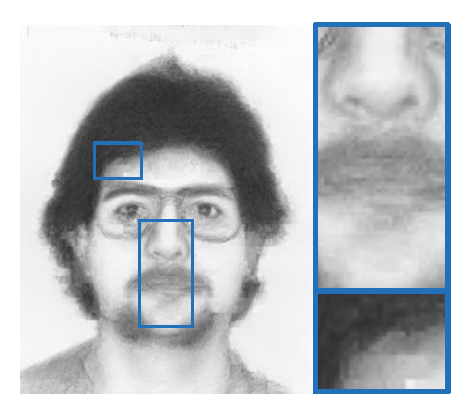
\includegraphics[width=0.99\linewidth]{img/sketch_result/example3_WMRF.pdf}
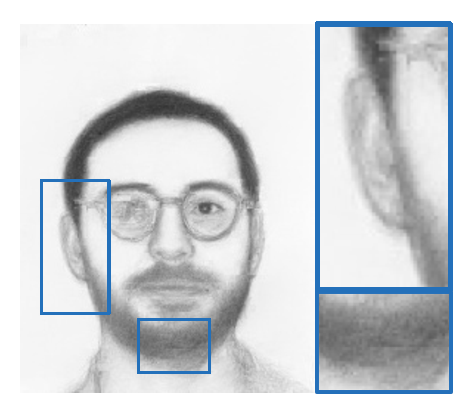
\includegraphics[width=0.99\linewidth]{img/sketch_result/example4_WMRF.pdf}
\end{minipage}
}
\subfigure[SSD]{
\begin{minipage}[b]{0.13\linewidth}
\centering
% \includegraphics[width=0.99\linewidth]{img/sketch_result/example1_SSD.pdf}
% \includegraphics[width=0.99\linewidth]{img/sketch_result/example2_SSD.pdf}
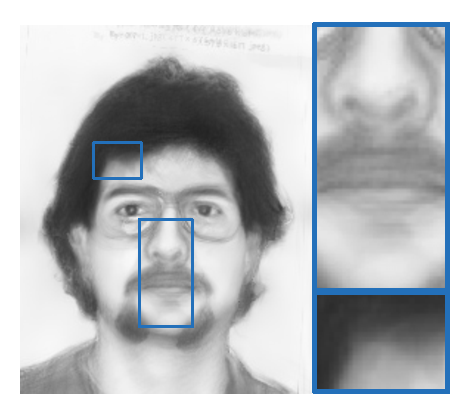
\includegraphics[width=0.99\linewidth]{img/sketch_result/example3_SSD.pdf}
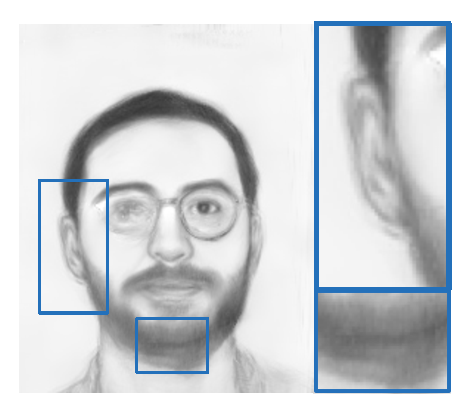
\includegraphics[width=0.99\linewidth]{img/sketch_result/example4_SSD.pdf}
\end{minipage}
}
\subfigure[FCNN]{
\begin{minipage}[b]{0.13\linewidth}
\centering
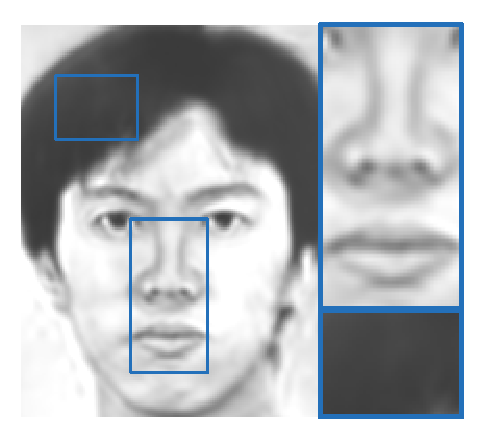
\includegraphics[width=0.99\linewidth]{img/sketch_result/example1_FCNN.pdf}
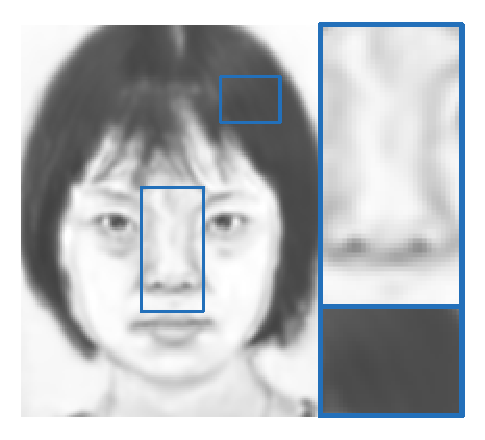
\includegraphics[width=0.99\linewidth]{img/sketch_result/example2_FCNN.pdf}
% \includegraphics[width=0.99\linewidth]{img/sketch_result/example3_FCNN.pdf}
% \includegraphics[width=0.99\linewidth]{img/sketch_result/example4_FCNN.pdf}
\end{minipage}
}
\subfigure[BFCN]{
\begin{minipage}[b]{0.13\linewidth}
\centering
% \includegraphics[width=0.99\linewidth]{img/sketch_result/example1_BFCN.pdf}
% \includegraphics[width=0.99\linewidth]{img/sketch_result/example2_BFCN.pdf}
% \includegraphics[width=0.99\linewidth]{img/sketch_result/example3_BFCN.pdf}
% \includegraphics[width=0.99\linewidth]{img/sketch_result/example4_BFCN.pdf}
\end{minipage}
}
\subfigure[Ours]{
\begin{minipage}[b]{0.13\linewidth}
\centering
\includegraphics[width=0.99\linewidth]{img/sketch_result/example1_ours.pdf}
\includegraphics[width=0.99\linewidth]{img/sketch_result/example2_ours.pdf}
\includegraphics[width=0.99\linewidth]{img/sketch_result/example3_ours.pdf}
\includegraphics[width=0.99\linewidth]{img/sketch_result/example4_ours.pdf}
\end{minipage}
}
\caption{Examples of qualitative evaluation on CUHK (first two rows) and AR (last two rows). (a) The sketches drawn by artists. (b) MRF~\cite{wang2009face} (c) WMRF~\cite{zhou2012markov} (d) SSD~\cite{song2014real} (e) FCNN~\cite{zhang2015end} (f) BFCN~\cite{zhang2017content} (g) Ours. The proposed method preserves more texture details, for example in the hair and nose. It is also best at keeping the origin structures of photos, such as the glasses.}
\label{fig:qua_eval}
\end{figure*}

\section{Experiments}

We evaluate the performance of the proposed method against other state-of-the-art methods on the CUHK student dataset~\cite{wang2009face} and the AR dataset~\cite{martinez1998r}. We compare the results of our method against other 6 methods including traditional approaches and recent deep learning models. After discussing the disadvantages of previous quantitative evaluation criteria, we introduce the Normalized Gram Matrix Difference (NGMD) as a new evaluation tool. We believe that NGMD is more effective and will greatly promote the sketch qualities in future work.
% those of the MRF method~\cite{wang2009face}, weighted MRF (WMRF) method~\cite{zhou2012markov}, feed-forward CNN (FCNN) method~\cite{zhang2017content,zhang2015end} and Filtering based method (SSD)~\cite{song2014real}.

%------------------------------------------------------------------------
\subsection{Style Transfer Evaluation}

Although style transfer has shown remarkable performance in artistic style, it can't be directly applied to face sketch synthesis, see Fig.~\ref{fig:example_h}. The generated sketch is greatly influenced by illumination of original photo and doesn't look like sketch at all. To prove our assumption in Section~\ref{sec:motivation} that gram matrix captures the density distribution of sketch, we replace the original RGB photo with content image generated by our content network. We selected 3 sketch styles with different amount of hairs and see how it influences the result. Fig.~\ref{fig:style_result} shows a clear relationship between the hair amount of sketch and pixel intensities of sketch result. The facial key parts in Fig.~\ref{fig:style_result2} and \ref{fig:style_result3} are missed. Therefore, even with a content structure, the original style transfer is still not suitable for elaborate task. However, if the style image has a similar structure with test photo, for example Fig.~\ref{fig:style_result1}, the results can be quite good. This inspires our feature patch based method. Image patch method is not considered because it will introduce patch inconsistency as discussed in Section~\ref{sec:related_work}. 

\begin{figure}[htbp]
\centering
\subfigure[]{
\label{fig:style_content} \includegraphics[width=0.23\linewidth]{img/style_evaluate/content.png}}
\subfigure[]{
\label{fig:style_result1} \includegraphics[width=0.23\linewidth]{img/style_evaluate/style_result1.pdf}}
\subfigure[]{
\label{fig:style_result2} \includegraphics[width=0.23\linewidth]{img/style_evaluate/style_result2.pdf}}
\subfigure[]{
\label{fig:style_result3} \includegraphics[width=0.23\linewidth]{img/style_evaluate/style_result3.pdf}}
\caption{(a) is the content image generated by our content network. (b), (c) and (d) are generated by different styles. It can be seen that when the hair decreases the generated sketch becomes brighter.}
\label{fig:style_result}
\end{figure}

%------------------------------------------------------------------------
\subsection{Sketch Generation}

Fig.~\ref{fig:qua_eval} shows the comparison between our methods and many other approaches. The first two rows are from CUHK test set, and the last two are from AR. We can see that our method can generate more stylistic sketches than others. For example, in the hair part, only MRF, BFCN and the proposed method can generate obvious textures. However, the texture of MRF is not continuous in the border part and introduce many other artifacts, and the texture of BFCN doesn't look like human strokes. Both WMRF and SSD introduce over smoothing effect and FCNN is not able to give clear textures. Our method can not only generate textures for hairs and mustache but also shadings, for example the nose part.

On the other hand, only BFCN and the proposed method can handle structures decorated on the face well, for example the glasses of the last two row. MRF, WMRF and SSD are exemplar based method so they can't handle something different from training set, the glass edges of them are not complete. FCNN, BFCN and our method generate the image content by CNN, so they can handle the original photo structures well. But both FCNN and BFCN care nothing about the textures of facial part, so their results are not good considering the face part. In contrast, our method can well maintain the image content and attach textures similar to human paintings. 

%------------------------------------------------------------------------
\subsection{Quantitative Results}

\paragraph*{Sketch Recognition} Sketch synthesis methods are usually evaluated quantitatively  via the face sketch recognition task~\cite{song2014real,wang2009face,zhang2015end,zhou2012markov}. If an algorithm achieves higher sketch recognition rates, it suggests that this method is more effective in synthesizing sketches. We adopt the widely used PCA based recognition method with ``rank-1 (R1)'', ``rank-5 (R5)'' and ``rank-10 (R10)'' criteria ~\cite{wang2009face} where ``rank $n$'' measures the rate of the correct answer in the top $n$ best matches. The results of different methods are shown in Table~\ref{tab:reg_percentage}. Our method achieves the best performance against all other methods in the ``R1'' and ``R5'' tests. 

% There may be two reasons behind this. First, since the test photos are different from those in the training set, we do not expect to find suitable patches from the training set for the target patches. The remedy of linearly combining the patches as in~\cite{zhou2012markov} will introduce over smoothing and blurring artifacts, which are also observed in the filtering like approach~\cite{song2014real}. Being a generative model, the content network learns the modality transformation locally between photos and sketches, such as transferring edges in photos to strokes in sketches. This helps generating sketches for structures not existing in the training set. Second, our model explicitly minimizes the difference by the 

\begin{table}[htbp]
\small
\begin{tabular}{C{0.2cm}C{0.2cm}C{0.35cm}C{0.1cm}C{0.35cm}C{0.1cm}C{0.35cm}C{0.1cm}C{0.35cm}C{0.1cm}C{0.35cm}C{0.1cm}C{0.35cm}}
\hline
\multicolumn{2}{c|}{\multirow {2}{*}{Methods}} & \multicolumn{5}{c}{AR} & & \multicolumn{5}{c}{CUHK} \\
\cline{3-7} \cline{9-13} \multicolumn{2}{c|}{} & R1 & & R5 & & R10 & & R1 & & R5 & & R10   \\
\hline
\multicolumn{2}{c|}{FCNN} & - & & - & & - & & 81\% & & 96\% & & 97\%   \\
\multicolumn{2}{c|}{MRF}  & 97.5\% & & 97.5\% & & \textcolor{red}{100\%} & & 83\% & & 96\% & & 96\% \\
\multicolumn{2}{c|}{WMRF} & 97.5\% & & 97.5\% & & \textcolor{red}{100\%} & & 83\% & & 97\% & & 98\%  \\
\multicolumn{2}{c|}{SSD}  & 96.7\% & & 97.5\% & & \textcolor{red}{100\%} & & \textcolor{red}{87\%} & & 97\% & & 98\%   \\
\multicolumn{2}{c|}{Ours} & \textcolor{red} {98.4\%} & & \textcolor{red} {98.4\%} & & \textcolor{red} {100\%} & & \textcolor{red} {87\%} & & \textcolor{red} {98\%} & & \textcolor{red} {99\%}   \\
\hline
\end{tabular}
\caption{Recognition rate on benchmark datasets. The best performance is colored in red.}
\label{tab:reg_percentage}
\end{table}

However, such kind of evaluation is not effective since every one is close to 100\%, and more importantly, it can't guide our research effort. Zhang \etal \cite{zhang2015end} proposed a  Multiscale Pixel-wise Reconstruction Loss (MPRL). Although we agree that if MPRL is zero, the generated sketches will be exactly the same with ground truth, there are two reasons why it is not a good criteria. First, experiment results of \cite{zhang2015end, zhang2017content} show that $L_2$-norm would give blurry sketches. Second, the ground truth draw by human usually doesn't correspond exactly with photos, thus difficult for algorithms to reach the ground truth.

Meanwhile, human can often be able to tell whether a sketch is generated by algorithms or drawn by artists just from a quick glance without examining details.
This indicates that there exists a big gap between the style of algorithm-generated sketches and that of those drawn by artists. And we need a criteria which can quantitatively measure such gap.

\paragraph*{Normalized Gram Matrix Difference (NGMD)} To quantitatively evaluate the style similarity between a generated sketch and the sketch drawn by a real artist, we employ the normalized gram matrix difference (NGMD) between the generated sketch $\mathcal{X}$ and the drawn sketch ${\tilde {\mathcal{X}}}$:
\begin{equation}
{D^l_s}\left( {\mathcal{X},\tilde {\mathcal{X}}} \right) = \frac{{\left\| {{G^l}\left( \mathcal{X} \right) - {G^l}\left( {\tilde {\mathcal{X}}} \right)} \right\|_2^2}}{{\left\| {{G^l}\left( {\tilde {\mathcal{X}}} \right)} \right\|_2^2}}
\label{eq:style_exp}
\end{equation}
where $l\in L_s$. The smaller the NGMD value is, the more similar $\mathcal{X}$ and ${\tilde {\mathcal{X}}}$ are. 
% Thanks to our style transfer, our results have the smallest NGMD value among all methods under test (see Table 2). It is therefore obvious that our results are the closest to the sketches drawn by artists. 
% Qualitative evaluation results are shown in Fig.~\ref{fig:qua_eval}, where we find that our method provides much clear boundaries and better texture in regions containing hairs and shadings. 

It is exciting how well NGMD match our intuition, see Fig.~\ref{fig:qua_eval}. 
The results of~\cite{zhang2015end} can roughly outline the sketches, thus they got a high NGMD in Table~\ref{tab:NGMD}. The results of MRF~\cite{wang2009face} and WMRF~\cite{zhou2012markov} are more similar to hand drawn sketches in style since these exemplar based approaches use patches of hand drawn sketches to make up the target sketch. That is why they have a smaller NGMD value. Inheriting the ability of denoising, the filtering based approach~\cite{song2014real} is good at suppressing noises in the results. However, it is also likely for this method to over-smooth the results, which will deteriorate the texture, thus its NGMD value is higher than WMRF. 

\begin{table*}[htbp]
\begin{center}
{\small
\begin{tabular}{ccccccccccccc}
\hline
\multicolumn{2}{c|}{\multirow {2}{*}{Methods}} &\multicolumn{5}{c}{AR} & & \multicolumn{5}{c}{CUHK} \\
\cline{3-7} \cline{9-13} \multicolumn{2}{c|}{} & conv1\_1 & conv2\_1 & conv3\_1 & conv4\_1 & conv5\_1 & &
 conv1\_1 & conv2\_1 & conv3\_1 & conv4\_1 & conv5\_1  \\
\hline
\multicolumn{2}{c|}{FCNN} & - & - & - & - & - & & { $0.009$} &{ $0.110$} & {$0.080$} & {$9.43$} & {$1.49$}  \\
\multicolumn{2}{c|}{MRF} & 0.0043 & 0.009 & {$0.033$}  & {$0.12$} & 0.28 & & { $0.010$} &{ $0.014$} & {$0.047$} & $0.13$ & $0.18$  \\
\multicolumn{2}{c|}{WMRF} & 0.0053 & 0.027 & {$0.085$}  & {$0.19$} & 0.29 & & { $0.010$} &{ $0.052$} & {$0.052$} & {$0.27$} & {$0.19$}  \\
\multicolumn{2}{c|}{SSD} & 0.0056 & 0.036 & {$0.110$} & {$1.90$} & 0.28 & & { $0.009$} &{ $0.102$} & {$0.070$} & {$3.32$} & {$0.24$}  \\
\multicolumn{2}{c|}{Ours} & {\color{red} 0.0035} & {\color{red} 0.008} & {\color{red} $0.029$} & {\color{red} $0.08$} & {\color{red} $0.17$} & & {\color{red}$0.007$} &{\color{red} $0.012$} & {\color{red} $0.033$} & {\color{red} $0.07$} & {\color{red} $0.12$}  \\
\hline
\end{tabular}
}
\end{center}
\caption{Averaged NGMD value of different methods at different level on AR and CUHK datasets. A smaller NGMD indicates the generated texture is more similar to ground truth.}
\label{tab:NGMD}
\end{table*}

%------------------------------------------------------------------------
\subsection{Generalization Evaluation}

In this part, we will evaluate the generalization ability of our model. Since the test photo may vary in pose and can't be well aligned, we just turn off the component loss. The parameters we use here are $\alpha=0.1$, $\beta_1=1$, $\beta_2=0$. 

\paragraph{Lightning and Pose Invariance} 

\paragraph{Real World Photos}


\begin{figure}[htbp]
\centering
\begin{minipage}[t]{0.49\linewidth}
\centering
\includegraphics[width=0.99\linewidth]{img/effective_eval/wo_region.pdf}
(a) $\beta_2=0$
\end{minipage}
\begin{minipage}[t]{0.49\linewidth}
\includegraphics[width=0.99\linewidth]{img/effective_eval/w_region.pdf}
\centering
(b) $\beta_2=0.1$
\end{minipage}
\caption{Comparison between results with and without the $\mathcal{L}_{k} $ regulation. (a) When turning off the component loss, the nose suffers from the distortion. (b) Thanks to the component loss, a more favorable result is obtained.}
\label{fig:region_effect}
\end{figure}

\begin{figure*}[htbp]
\centering
\begin{minipage}[t]{0.16\linewidth}
\centering
\includegraphics[width=0.99\linewidth]{img/effective_eval/inf_alpha.pdf}
$\beta_1  = 0 $\\
$\beta_2  = 0 $
\end{minipage}
\begin{minipage}[t]{0.16\linewidth}
\centering
\includegraphics[width=0.99\linewidth]{img/effective_eval/4_alpha.pdf}
$\beta_1  = 10^{-3} $\\
$\beta_2  = 10^{-4} $
\end{minipage}
\begin{minipage}[t]{0.16\linewidth}
\centering
\includegraphics[width=0.99\linewidth]{img/effective_eval/3_alpha.pdf}
$\beta_1  = 10^{-2} $\\
$\beta_2  = 10^{-3} $
\end{minipage}
\begin{minipage}[t]{0.16\linewidth}
\centering
\includegraphics[width=0.99\linewidth]{img/effective_eval/2_alpha.pdf}
$\beta_1  = 0.1 $\\
$\beta_2  = 0.01 $
\end{minipage}
\begin{minipage}[t]{0.16\linewidth}
\centering
\includegraphics[width=0.99\linewidth]{img/effective_eval/1_alpha.pdf}
$\beta_1  = 1 $\\
$\beta_2  = 0.1 $
\end{minipage}
\begin{minipage}[t]{0.16\linewidth}
\centering
\includegraphics[width=0.99\linewidth]{img/effective_eval/0_alpha.pdf}
$\beta_1  = 10^{3} $\\
$\beta_2  = 10^{2} $
\end{minipage}
\caption{Final results for sketch synthesis with fixed $\alpha=0.004$ and different $\beta_1$, $\beta_2$ values.}
\label{fig:alphg_effect}
\end{figure*}

%------------------------------------------------------------------------
\subsection{Effectiveness of the model}

The loss function we minimize during the generation of sketches contains three terms for content, style and key components respectively. The term $\mathcal{L}_{k} $ regularizes the results by encouraging the style extracted from the key component regions in the training set to be placed into the key components region of the results, which helps generate better results around these components (see Fig.~\ref{fig:region_effect}). To better understand how style influences the final sketch, we smoothly change the emphasis on style by adjusting $\beta_1$ and $\beta_2$ while keeping $\alpha$  fixed. Fig.~\ref{fig:alphg_effect} indicates that the sketch with style transfered contains more texture and is more like a drawn sketch. The Theano implementation of the proposed method takes approximately $100$ seconds to generate a sketch on a GeForce GTX TITAN X platform. The bottle neck lies in the style transfer which requires feeding $\mathcal{X}$ to the VGG-Network to estimate targeting feature maps and to calculate the gradient of Eq.~(\ref{eq:Total_loss}), which is computationally intensive. 

%==========================================================================
\section{Conclusion}

This paper proposed a novel face sketch synthesis method inspired by the procedure of artists drawing sketches. In our method, the outline of the face is delineated by a content network and the style extracted from sketches drawn by artists are transferred to generate a final sketch. Quantitative evaluations on face sketch recognition and style similarity measure demonstrate the effectiveness of the proposed algorithm for face sketch synthesis and style transferring. Our future work will investigate accelerating technique to reduce the running time and achieve real time face sketch synthesis with style transfer.


{\small
\bibliographystyle{ieee}
\bibliography{egbib}
}

\end{document}
